%% prezentacia.tex
%% Copyright 2016, 2017 Juraj Szasz <juraj.szasz3@gmail.com>
%
% This work may be distributed and/or modified under the conditions of the LaTeX
% Project Public License, either version 1.3 of this license or (at your option)
% any later version.  The latest version of this license is in
%   http://www.latex-project.org/lppl.txt
% and version 1.3 or later is part of all distributions of LaTeX version
% 2005/12/01 or later.
%
% This work has the LPPL maintenance status `author-maintained'.
%
% This work consists of the following files: diplomovka.tex, 01-uvod.tex,
% 02-symboly.tex, 03-kapitola1.tex, 04-kapitola2.tex, 05-kapitola3.tex,
% 06-zaver.tex, 07-priloha.tex, literatura.bib, opakuj.sty, ucmthesis.sty and
% ucmplainnat.bst.
%
% The file `ucmplainnat.bst' was derived from the `csplainnat.bst' BibTeX style
% for Czech references style (According to CSN ISO 690) available at:
%   https://github.com/mudrd8mz/csplainnat
%
% All the other files above were derived from the Masaryk University, Faculty of
% Science template available for download at:
%   http://www.sci.muni.cz/NW/STUD/SablonyPraci/Sablona_Pruvodce_(v1.9).zip
%
%%%%%%%%%%%%%%%%%%%%%%%%%%%%%%%%%%%%%%%%%%%%%%%%%%%%%%%%%%%%%%%%%%%%%%%%%%%%%%%%
%%
%%  Sablona Bc+Mgr+RNDr pre FPV UCM
%%  Autor: Juraj Szasz (juraj.szasz3@gmail.com)
%%
%%  Zalozene na sablone PriF MU v Brne
%%    Autor: Petr Zemanek (zemanekp@math.muni.cz)
%%
%%  Typeset in LaTeX-2e
%%
%%%%%%%%%%%%%%%%%%%%%%%%%%%%%%%%%%%%%%%%%%%%%%%%%%%%%%%%%%%%%%%%%%%%%%%%%%%%%%%%

%\documentclass[12pt,a4paper,oneside,final]{book}
\documentclass{beamer}
\usetheme{default} % pouzitie default temy
\setbeamertemplate{frametitle}[default][center]

\usepackage[utf8]{inputenc}
\usepackage[LGR,IL2]{fontenc}
\usepackage[english,slovak]{babel} % posledny jazyk v zozname je implicitny

\usepackage{mathptmx}  % volne dostupny font Adobe Times Roman

\usepackage{longtable} % balik pre tabulky presahujuce jednu stranu
                       % (potrebne pre zoznam znaceni)

\usepackage{booktabs}  % balík pre vysadzanie profesionalnych tabuliek

% balik pre postranne popisky obrazkov a tabuliek
\usepackage[leftcaption,ragged]{sidecap}

\usepackage{amsmath,amssymb,amsthm} % baliky pre matematicke vzorce
\usepackage{natbib}    % balik pre harvardsky styl citacii

\usepackage{gfsporson} % balik pre vysadzanie greckeho textu
\usepackage{fancyvrb}  % balik pre oramovanie verbatim prostredia
\usepackage{tabularx}
%\usepackage{colorx}    % balík pre farebný text

%%%%%%%%%%%%%%%%%%%%%%%%%%%%%%%%%%%%%%%%%%%%%%%%%%%%%%%%%%%%%%%%%%%%%%%%%%%%%%%%
%%
%%  Nastavenie stylu citacii
%%
%%%%%%%%%%%%%%%%%%%%%%%%%%%%%%%%%%%%%%%%%%%%%%%%%%%%%%%%%%%%%%%%%%%%%%%%%%%%%%%%
\bibliographystyle{ucmplainnat}
\setcitestyle{authoryear}

%%%%%%%%%%%%%%%%%%%%%%%%%%%%%%%%%%%%%%%%%%%%%%%%%%%%%%%%%%%%%%%%%%%%%%%%%%%%%%%%
%%
%%  Nastavenie sablony
%%
%%%%%%%%%%%%%%%%%%%%%%%%%%%%%%%%%%%%%%%%%%%%%%%%%%%%%%%%%%%%%%%%%%%%%%%%%%%%%%%%

%\usepackage[Mgr,Farebne]{ucmthesis}   % nahrad "Farebne" za "Tlac", ked chces
                                      % dokument tlacit; "Farebne" je len pre
                                      % zdielanie online

\graphicspath{{obr/}}                 % implicitna cesta pre umiestnenie
                                      % obrazkov v adresari 'obr'

\author{Bc. Juraj Szász}

\title{Scientometrická analýza FPV~UCM v~Trnave}

\date{\today}

%\NazovKatedry{Katedra biológie}{Department of Biology}

%\MiestoRieseniaPrace{Trnava}{Trnava}

%\AkademickyRok{2016/2017}

%\SkolitelSTitulmi{prof. RNDr. Ján Kraic, PhD}

%\StudijnyProgram{Aplikovaná biológia}{Aplicated Biology}

%\StudijnyObor{Biológia}{Biology}


%\TextAbstraktov{Scientometrická analýza slúži na kvalitatívne a~kvantitatívne
% hodnotenie vedeckej práce.  Vykonáva sa pomocou štatistickej analýzy
% publikačnej činnosti jednotlivých pracovníkov, inštitúcií a~dokonca celých
% krajín.  Kvalitu vedeckých publikácií určuje množstvo citácií (odkazov) na
% publikácie.  Viac citácií na článok vyjadruje jeho popularitu, kvalitu
% a~prínos pre vedecký pokrok.  Cieľom tejto práce je kvalitatítne
% a~kvantitatívne zhodnotiť publikačnú činnosť pracovníkov Fakulty prírodných
% vied Univerzity sv.\,Cyrila a Metoda v~Trnave za~obdobie 2000--2016.}{The
% purpose of scientometric analysis is to provide qualitative and quantitative
% evaluation of the scientific work.  It is being performed by statistical
% analysis of the publishing activity---addressing individual researchers,
% institutions or even whole countries.  The quality of a scientific publication
% is derived from the number of citations.  The amount of references to a paper
% determines its popularity, quality and its impact on scientific progress.  The
% goal of this thesis is to carry out qualitative and quantitative analysis of
% the publishing activity of the academic staff members affiliated to Faculty of
% Natural Science, University of Ss.\,Cyril and Methodeus in Trnava during
% 2000--2016.}

%%%%%%%%%%%%%%%%%%%%%%%%%%%%%%%%%%%%%%%%%%%%%%%%%%%%%%%%%%%%%%%%%%%%%%%%%%%%%%%%
%%
%% Definícia vlastných príkazov
%%
%%%%%%%%%%%%%%%%%%%%%%%%%%%%%%%%%%%%%%%%%%%%%%%%%%%%%%%%%%%%%%%%%%%%%%%%%%%%%%%%

\newcommand{\Cbb}{\mathbb{C}}
\newcommand{\Rbb}{\mathbb{R}}
\newcommand{\Zbb}{\mathbb{Z}}
\newcommand{\Nbb}{\mathbb{N}}
\newcommand{\tm}{\texttrademark}
\newcommand{\R}{\textsuperscript{\textregistered}}

% Environment for source code
\newenvironment{source}[1][\scriptsize\bfseries]{
  \begin{list}{}{
      \setlength{\leftmargin}{1em}}%
      \setlength{\itemsep}{0pt}%
      \setlength{\parskip}{0pt}%
      \setlength{\parsep}{0pt}%
      \renewcommand{\baselinestretch}{1.0}%
  \item#1}
  {\end{list}}
%%%%%%%%%%%%%%%%%%%%%%%%%%%%%%%%%%%%%%%%%%%%%%%%%%%%%%%%%%%%%%%%%%%%%%%%%%%%%%%%
%%
%%  Dodatocne nastavenia
%%
%%%%%%%%%%%%%%%%%%%%%%%%%%%%%%%%%%%%%%%%%%%%%%%%%%%%%%%%%%%%%%%%%%%%%%%%%%%%%%%%

% Vytvori pomocny subor pre register
%\makeindex

% Zapnutie opakovania matematickych symbolov
% %Podle Tesaříkova czech.ldf
\makeatletter
\def\Deleni{%
 \ifx\protect\@typeset@protect
   \ifhmode
     \ifinner
       \bbl@afterelse\bbl@afterelse\bbl@afterelse\cs@hyphen
     \else
       \bbl@afterfi\bbl@afterelse\bbl@afterelse\cs@firsthyphen
     \fi
   \else
     \bbl@afterfi\bbl@afterelse\cs@hyphen
   \fi
 \else
   \bbl@afterfi\cs@hyphen
 \fi }
\makeatother

%Opakování symbolů binárních operací a relací při zalomení řádku
%Autor: Josef Tkadlec tkadlec@fel.cvut.cz

\relpenalty     =10000      % aby se nelámalo v jiných než ošetřených
\binoppenalty   =10000
\exhyphenpenalty=1000       % aby spíše nouzově (implicitně je 50)
                           % "lokálně" lze zakázat {...}

\def\neq {\mathrel{\not=}}  % aby nedocházelo k lámání \not=/=
\let\ne=\neq

\def\OpakujPrikaz #1#2{\let #2=#1
 \def #1{#2\nobreak\discretionary{}{\hbox{$#2$}}{}}}
\def\OpakujZnak #1#2{\mathchardef #2=\mathcode`#1
 \activedef #1{#2\nobreak\discretionary{}{\hbox{$#2$}}{}}
 \uccode`\~=0 \mathcode`#1="8000 }
%Doplnil Kuben pro nový czech.ldf \expandafter možná nemusí být
\def\OpakujZnakMinus #1#2{\mathchardef #2=\mathcode`#1
 \activedef #1{\ifmmode#2\nobreak\discretionary{}{\hbox{$#2$}}{}\else\expandafter\Deleni\fi }
 \uccode`\~=0 \mathcode`#1="8000 }
\def\activedef #1{\uccode`\~=`#1 \uppercase{\def~}}

\OpakujPrikaz {\neq }{\neqORI}  \let \ne=\neq
\OpakujPrikaz {\leq }{\leqORI}  \let \le=\leq
\OpakujPrikaz {\geq }{\geqORI}  \let \ge=\geq
\OpakujPrikaz {\cup }{\cupORI}
\OpakujPrikaz {\cap }{\capORI}
\OpakujPrikaz {\times }{\timesORI}
\OpakujPrikaz {\subset }{\subsetORI}
\OpakujPrikaz {\subseteq }{\subseteqORI}
\OpakujPrikaz {\supset }{\supsetORI}
\OpakujPrikaz {\supseteq }{\supseteqORI}

\OpakujPrikaz {\cdot }{\cdotORI}
\OpakujPrikaz {\setminus }{\setminusORI}

\OpakujZnak <{\lessORI}
\OpakujZnak >{\greaterORI}
\OpakujZnak +{\plusORI}
\AtBeginDocument {\OpakujZnak ={\eqORI} \OpakujZnakMinus -{\minusORI}}

%%%%%%%%%%%%%%%%%%%%%%%%%%%%%%%%%%%%%%%%%%%%%%%%%%%%%%%%%%%%%%%%%%%%%%%%%%%%%%%%
%%
%%  Zaciatok dokumentu
%%
%%%%%%%%%%%%%%%%%%%%%%%%%%%%%%%%%%%%%%%%%%%%%%%%%%%%%%%%%%%%%%%%%%%%%%%%%%%%%%%%

\begin{document}

%%
%%  Uvodna strana
%%

\frame{\maketitle}

\frame{\tableofcontents}

\begin{frame}
  \frametitle{Definície}
  \framesubtitle{Scientometria}
  \begin{itemize}
    \item Scientometria je hodnotenie vedy (publikácií, pracovníkov,
      inštitúcií, až krajín) použitím matematických a štatistickým metód
      \citep{Vinkler2001}.
    \item Základ hodnotenia tvorí počet referencíí na publikáciu tzv. citácie.
      Pričom táto hodnota predstavuje impakt (dopad) daného dokumentu na vedu,
      teda kvalitu \citep{Vavrikova2008}.
    \item V scientometrie sa môže hodnotiť aj ekonomický aspekt vedeckého
      výskumu (napr. financovanie inštitúcií a grantov). Ale väčšiu váhu má
      hodnotenie na základe citácií, pretože financovanie samo o sebe nič
      nehovorí o dopade daného objavu \citep{Bellis2009}.
    %\item Kvalitu vedeckých publikácií na internete je možné hodnotiť na základe frekvencie 
    %  počtu prístupov na ne. Tento aspekt skúma cybermetria (resp. webometria).
  \end{itemize}
\end{frame}

%\begin{frame}
  %\frametitle{Celkový počet publikácií jednotlivých katedier FPV UCM v~Trnave}
%  \frametitle{Definície}
%  \framesubtitle{Vzťah medzi disciplínami v rámci informetrie}
  %\framesubtitle{Celkový počet publikácií jednotlivých katedier}
%  \begin{figure}
%    \centering
%    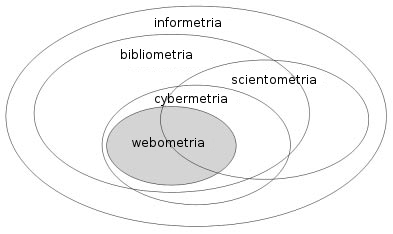
\includegraphics[scale=0.5]{fields.png}
%    \caption{\citep{Bjorneborn2004}}
%  \end{figure}
%\end{frame}

\begin{frame}
  \frametitle{Definície}
  \framesubtitle{Výber citačných indikátorov použitých v diplomovej práci}

  \centering\small
  \begin{table}
  \begin{tabularx}{\textwidth}{llccr}
    \toprule\noalign{\vspace{.3ex}}
    slovenský  názov                     & anglický názov                         & skratka                 & kap.                 \\[0.3ex]
    \midrule\noalign{\vspace{.5ex}}
    {\color{red} impakt faktor}          & {\color{red}\emph{Journal Impact Factor}}           & IF                      &  1.5.1        \\[0.5ex]
    {\color{red} SciMago rang časopisu}  & {\color{red}\emph{SciMago Journal Rank}}            & SJR                     &  1.5.2       \\[0.5ex]
    {\color{red}CiteScore}$^\dagger$     & {\color{red}\emph{CiteScore}}                       & CS                      &  1.5.3       \\[0.5ex]
    {\color{red}normalizovaný impakt}    & {\color{red}\emph{Source normalized impact}}        & SNIP                    &  1.5.4      \\[-0.25ex]
    {\color{red}časopisu  na dokument}   & {\color{red}\emph{per paper}}                       &                         &                       \\[0.5ex]
    Hirschov index                       & \emph{Hirsh's index}                   & $h$-index               &  1.6.1    \\[1.5ex]
    Eggheov index                        & \emph{Egghe's index}                   & $g$-index               &  1.6.2    \\[0.5ex]
    \bottomrule \\ [-2ex]
    \multicolumn{5}{l}{\footnotesize {\color{red} červenou farbou} sú označené citačné indikátory na hodnotenie časopisov} \\
    \multicolumn{5}{l}{\footnotesize $^\dagger$ indikátory, ktorých názov sa neprekladá so slovenčiny}
  \end{tabularx}
    \caption{\citet{Szasz2017}}
  \end{table}
\end{frame}

\begin{frame}
  \frametitle{Praktická časť}
  \framesubtitle{Program Publish or Perish}
  \begin{figure}
    \centering
    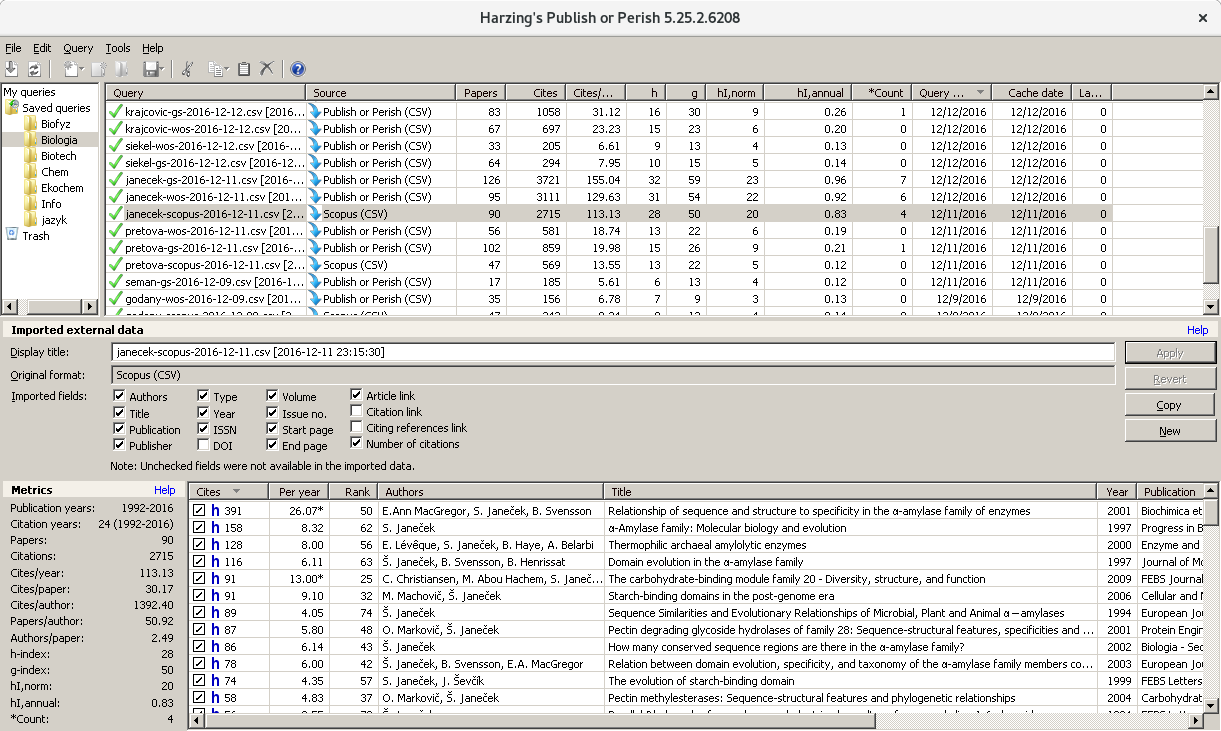
\includegraphics[scale=0.25]{publish-or-perish_wine.png}
    \caption{\citet{Harzing2011}}
  \end{figure}
\end{frame}

\begin{frame}
  %\frametitle{Celkový počet publikácií jednotlivých katedier FPV UCM v~Trnave}
  \frametitle{Výsledky}
  \framesubtitle{Celkový počet publikácií jednotlivých katedier FPV UCM v~Trnave}
  %\framesubtitle{Celkový počet publikácií jednotlivých katedier}
  \begin{figure}
    \centering
    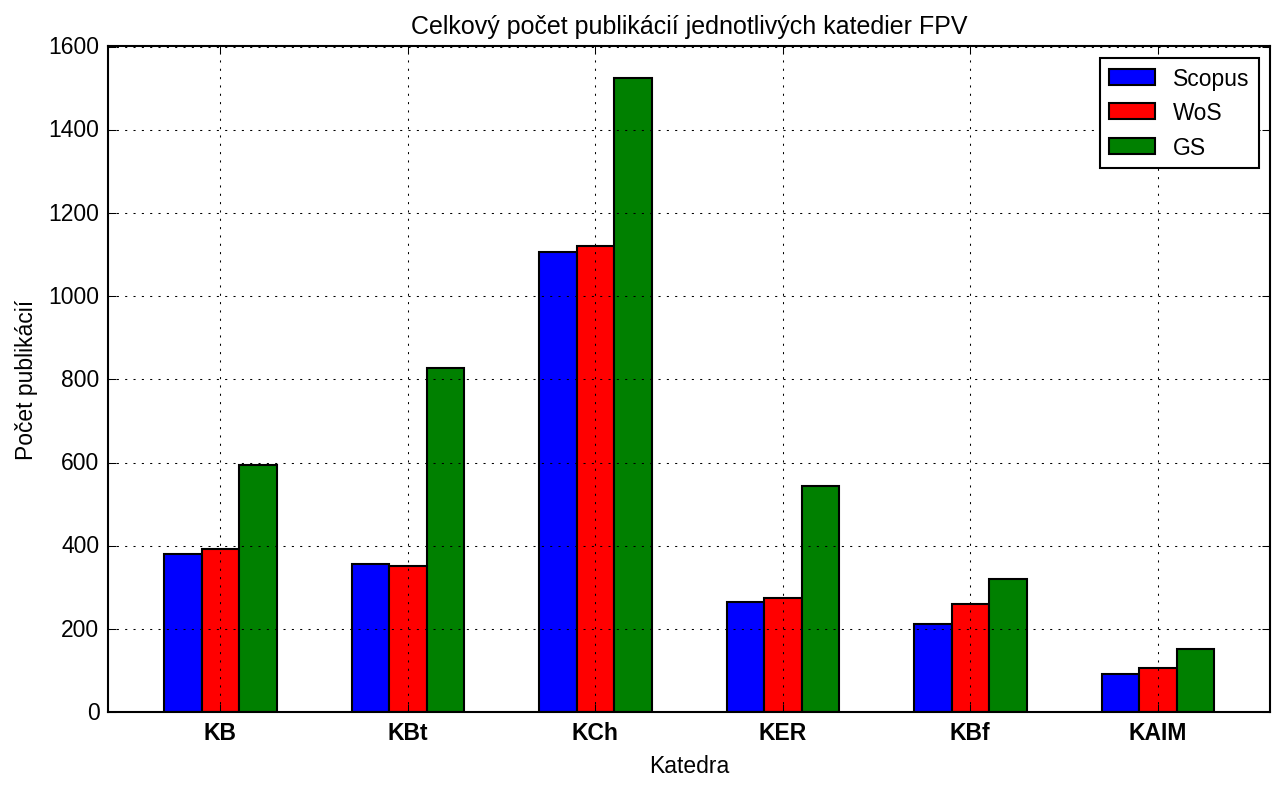
\includegraphics[scale=0.5]{plot-results-data-papers.png}
  \end{figure}
\end{frame}

\begin{frame}
  \frametitle{Výsledky}
  \framesubtitle{Celkový počet citácií jednotlivých katedier FPV UCM v~Trnave}
  %\framesubtitle{Celkový počet citácií jednotlivých katedier}
  \begin{figure}
    \centering
    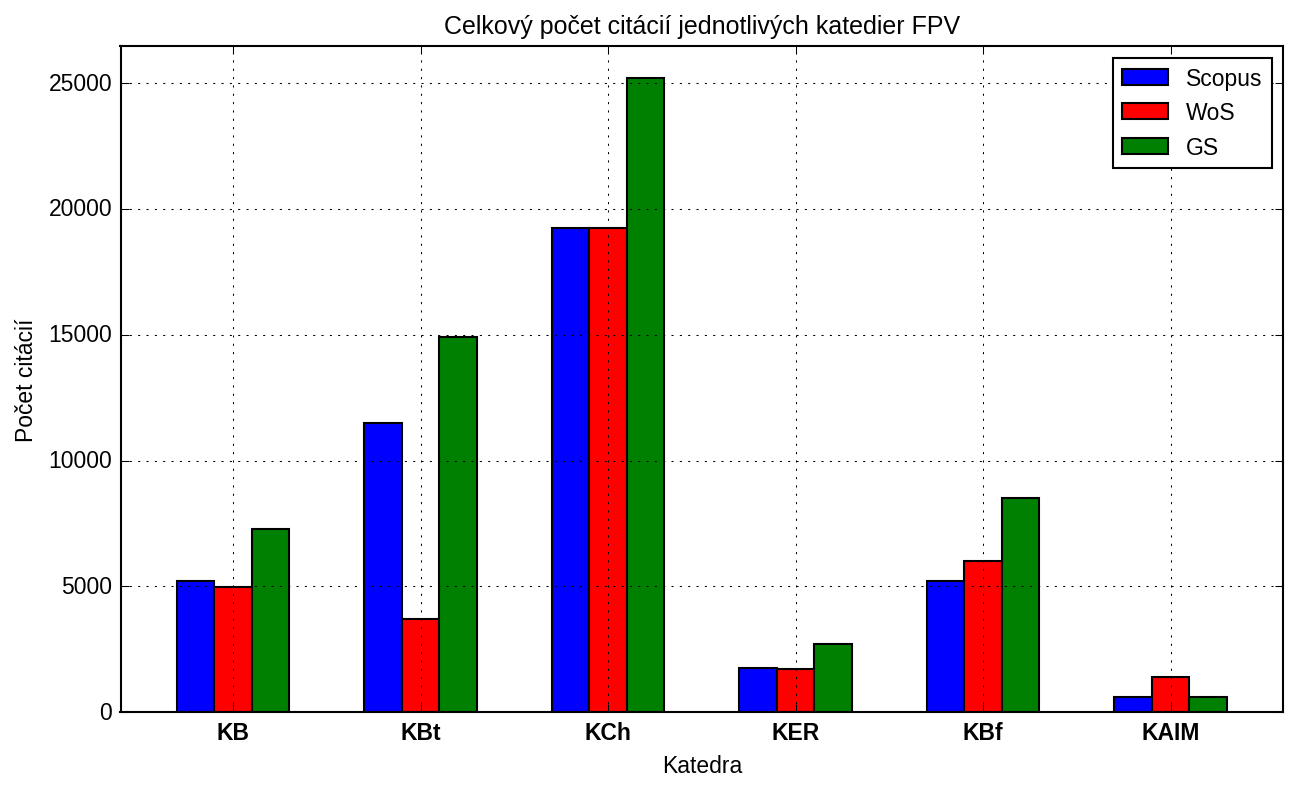
\includegraphics[scale=0.5]{plot-results-data-citations.png}
  \end{figure}
\end{frame}

\begin{frame}
  \frametitle{Výsledky}
  \framesubtitle{Medián $h$-indexu pre jednotlivé katedry FPV UCM v~Trnave}
  %\framesubtitle{Medián $h$-indexu pre jednotlivé katedry}
  \begin{figure}
    \centering
    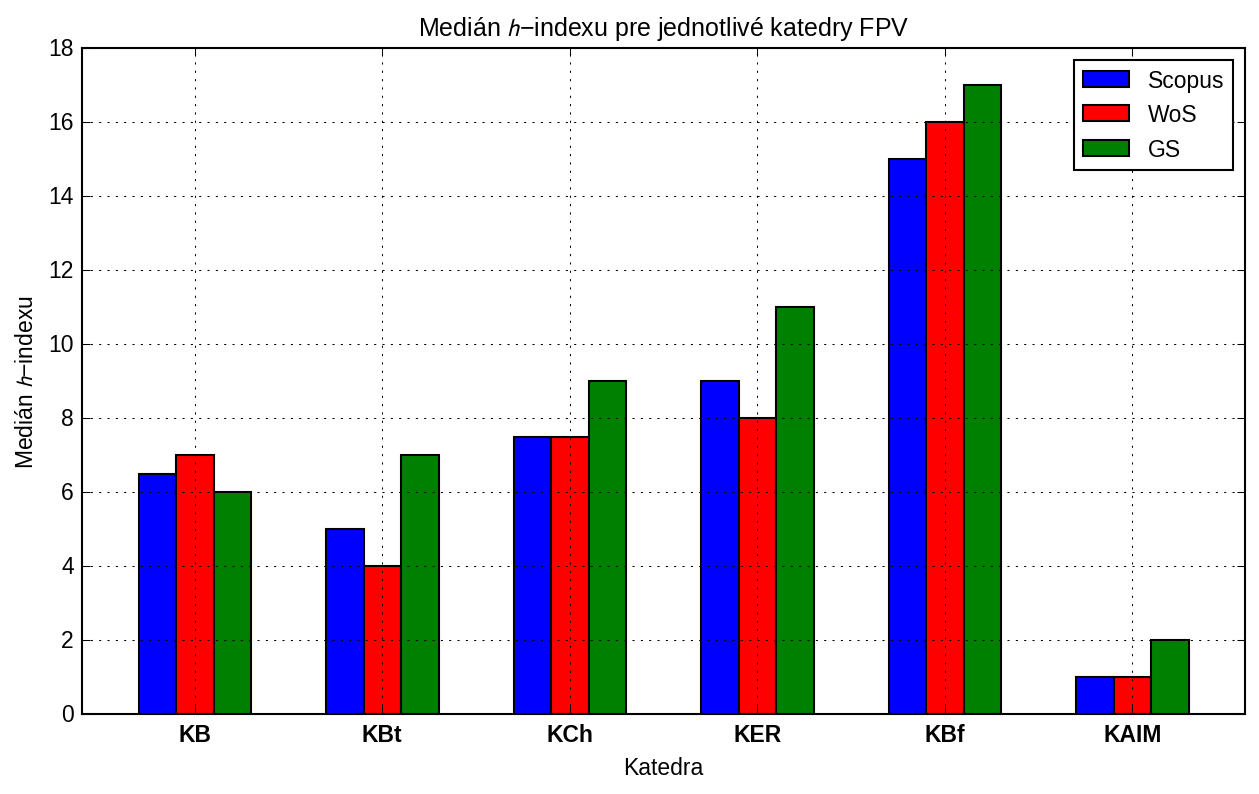
\includegraphics[scale=0.5]{plot-results-data-h_index.png}
  \end{figure}
\end{frame}

\begin{frame}
  \frametitle{Výsledky}
  \framesubtitle{Medián $g$-indexu pre jednotlivé katedry FPV UCM v~Trnave}
  %\framesubtitle{Medián $g$-indexu pre jednotlivé katedry}
  \begin{figure}
    \centering
    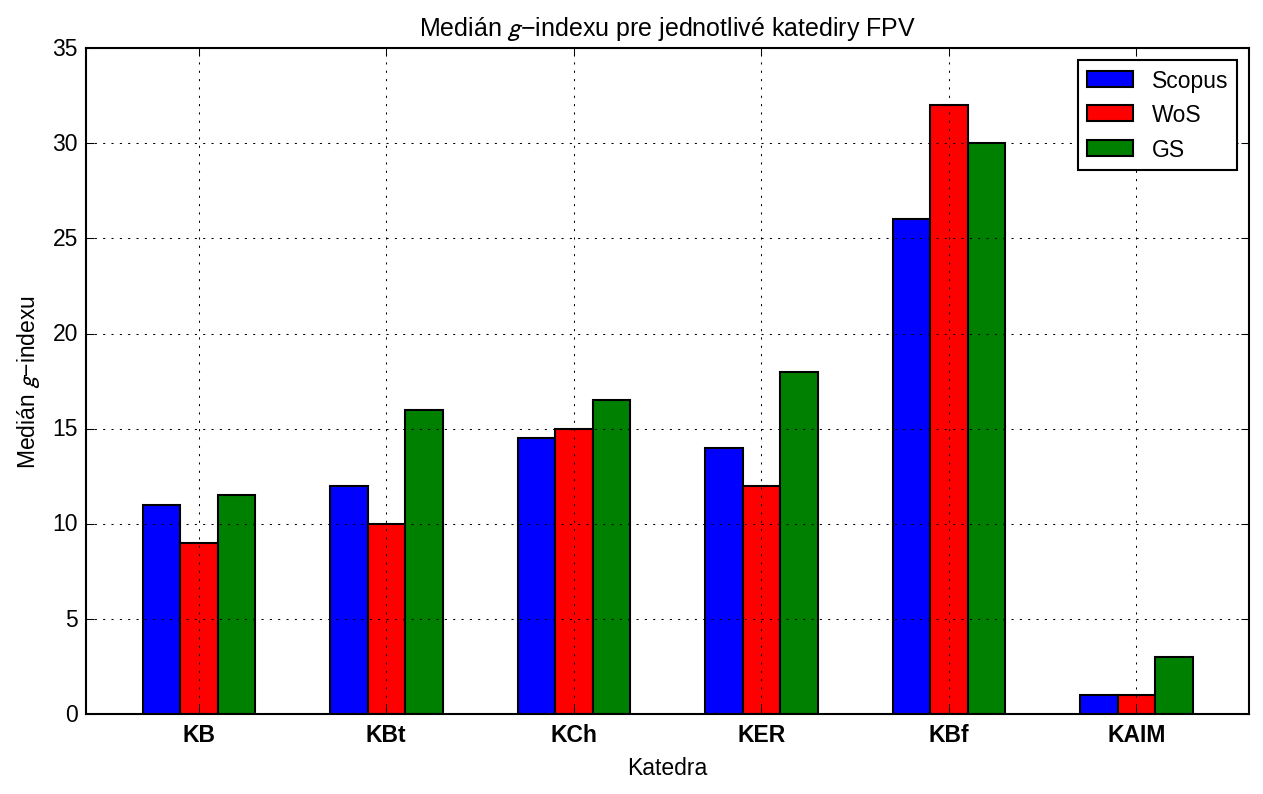
\includegraphics[scale=0.5]{plot-results-data-g_index.png}
  \end{figure}
\end{frame}

\begin{frame}
  \frametitle{Výsledky}
  \framesubtitle{Svetové časopisy s najväčším počtom publikácií z FPV UCM v~Trnave}
  \vspace{-0.5em}

  {\small
  \begin{tabular}{lcccccc}
    %\caption*{Prehľad časopisov, v~ktorých publikovali pracovníci FPV UCM v~Trnave.}
    \toprule\noalign{\vspace{.3ex}}
     %\hline
     Názov časopisu                                                                   & $n^\dagger$ & IF & SJR  & CS$^\ddagger$ & SNIP           \\[0.3ex]
   \midrule\noalign{\vspace{.5ex}}
     % \hline

    Chemical Papers                                                                    & 25     & 1.326   & 0.382 &  1.36      & 0.56                  \\
    Polyhedron                                                                         & 22     & 2.108   & 0.592 &  2.02      & 0.777                 \\
    Biologia                                                                           & 15     & 1,10    & 0.322 &  0.88      & 0.88                  \\
    Cereal Research Communications                                                     & 14     & 0.528   & 0.305 &  0.62      & 0.515                 \\
    Dalton Transactions                                                                & 14     & 4.177   & 1.404 &  4.1       & 1                     \\[1ex]
    Chemicke Listy                                                                     & 13     & 0.279   & 0.183 &  0.22      & 0.24                  \\
    Inorganic Chemistry                                                                & 12     & 4.82    & 1.873 &  1.36      & 0.741                 \\
    Inorganica Chimica Acta                                                            & 11     & 1.918   & 0.584 &  1.88      & 0.664                 \\
    Nova Biotechnologica et Chimica                                                    & 11     & 0.188   & 0.129 &  0.31      & 0.044                 \\
    \bottomrule \\ [-2ex]
    \multicolumn{7}{l}{\footnotesize $^\dagger$ Počet publikácií pracovníkov FPV; $^\ddagger$ CiteScore} \\
     
  \end{tabular}}

  Zdroj Scopus a Web of Science (2000-2016)

\end{frame}

\begin{frame}
  \frametitle{Iné zdroje impakt faktoru}
  \begin{tabular}{llll}
    \hline
    Časopis                                            & ISI JIF & IF    & zdroj                                                                                             \\
    Polish Journal of Environmental Studies            & 0,79    & 0,71  & https://www.researchgate.net/journal/1230-1485\_Polish\_Journal\_of\_Environmental\_Studies            \\
    Pharmazie                                          & 1.264   & 1.32  & https://www.researchgate.net/journal/0031-7144\_Pharmazie                                          \\
    Applied Mechanics and Materials                    &         & 0.16  & https://www.researchgate.net/journal/1660-9336\_Applied\_Mechanics\_and\_Materials                    \\
    Advanced Materials Research                        &         & 0.23  & https://www.researchgate.net/journal/1662-8958\_Advanced\_Materials\_Research                        \\
    Nova Biotechnologica et Chimica                    &         & 0.188$^\dagger$ & https://www.degruyter.com/view/j/nbec                                                             \\
    Communications in computer and information science &         & 0.35  & https://www.researchgate.net/journal/1865-0929\_Communications\_in\_Computer\_and\_Information\_Science \\
    \hline
    \multicolumn{4}{l}{\footnotesize $^\dagger$ Hodnota nie je impakt faktor, ale impakt na publikáciu (IPP)} \\
  \end{tabular}
\end{frame}

%%
%%  Zoznam pouzitej literatury
%%
\begin{frame}
  \frametitle{Zoznam literatúry}
\bibliography{literatura}{}
\end{frame}

\end{document}

